\documentclass[9pt,twocolumn,twoside,lineno]{pnas-new}
% Use the lineno option to display guide line numbers if required.
\usepackage{subcaption}
\templatetype{pnasresearcharticle} % Choose template 

\title{Universal front-end gain control aids robust combinatorial coding in naturalistic environments}

% Use letters for affiliations, numbers to show equal authorship (if applicable) and to indicate the corresponding author
\author[a]{Nirag Kadakia}
\author[a,b]{Thierry Emonet} 

\affil[a]{Department of Molecular, Cellular, and Developmental Biology}
\affil[b]{Department of Physics, Yale University, New Haven, CT 06511}

% Please give the surname of the lead author for the running footer
\leadauthor{Kadakia} 

% Please add here a significance statement to explain the relevance of your work
\significancestatement{In insect olfaction, odors are believed to be encoded by the distinct spatiotemporal patterns of activity they elicit in sensing neurons. Here, we investigate how these patterns would be maintained in naturalistic environments, where odor concentrations can vary rapidly, and where ethologically-relevant odors often mix with nuisance backgrounds. Here, we show that a single, robust mechanism of response adaptation, Weber’s Law of perceived difference, which was recently observed in \textit{Drosophila}, may play a vital role in maintaining these odor codes. While Weber's Law is known to maintain sensitivity in single-channel systems such as bacterial chemotaxis, here we illustrate its general applicability to multi-channels systems in which responses may be broad and highly overlapping.}

% Please include corresponding author, author contribution and author declaration information
\authorcontributions{Please provide details of author contributions here.}
\authordeclaration{Please declare any conflict of interest here.}
\equalauthors{\textsuperscript{1}A.O.(Author One) and A.T. (Author Two) contributed equally to this work (remove if not applicable).}
\correspondingauthor{\textsuperscript{2}To whom correspondence should be addressed. E-mail: author.two\@email.com}

% Keywords are not mandatory, but authors are strongly encouraged to provide them. If provided, please include two to five keywords, separated by the pipe symbol, e.g:
\keywords{Odor coding $|$ Drosophila olfaction $|$ Sensory systems $|$ Weber's Law $|$ Olfactory receptor neurons} 

\begin{abstract}
	Please provide an abstract of no more than 250 words in a single paragraph. Abstracts should explain to the general reader the major contributions of the article. References in the abstract must be cited in full within the abstract itself and cited in the text.Please provide an abstract of no more than 250 words in a single paragraph. Abstracts should explain to the general reader the major contributions of the article. References in the abstract must be cited in full within the abstract itself and cited in the text.Please provide an abstract of no more than 250 words in a single paragraph. Abstracts should explain to the general reader the major contributions of the article. References in the abstract must be cited in full within the abstract itself and cited in the text.Please provide an abstract of no more than 250 words in a single paragraph. Abstracts should explain to the general reader the major contributions of the article. References in the abstract must be cited in full within the abstract itself and cited in the text.Please provide an abstract of no more than 250 words in a single paragraph. Abstracts should explain to the general reader the major contributions of the article. References in the abstract must be cited in full within the abstract itself and cited in the text.Please provide an abstract of no more than 250 words in a single paragraph. Abstracts should explain to the general reader the major contributions of the article. 
\end{abstract}

\dates{This manuscript was compiled on \today}
\doi{\url{www.pnas.org/cgi/doi/10.1073/pnas.XXXXXXXXXX}}

% Added to get write linespread as published articles
\linespread{0.9}
\begin{document}


% Optional adjustment to line up main text (after abstract) of first page with line numbers, when using both lineno and twocolumn options.
% You should only change this length when you've finalised the article contents.
%\verticaladjustment{-2pt}

\maketitle
\thispagestyle{firststyle}
\ifthenelse{\boolean{shortarticle}}{\ifthenelse{\boolean{singlecolumn}}{\abscontentformatted}{\abscontent}}{}

%%%%%%%%%%%%%%%%%%%%%%%%%%%%%%%%%%%%%%%%%%%%%%%%%%%%%%%%%%%%%%%%%
%%%%%%%%%%%%    		INTRODUCTION	    		%%%%%%%%%%%%%
%%%%%%%%%%%%%%%%%%%%%%%%%%%%%%%%%%%%%%%%%%%%%%%%%%%%%%%%%%%%%%%%%




Animals identify and discriminate odors using olfactory receptors (Ors) expressed in olfactory receptor neurons (ORNs)~\cite{Or_ORNs_maps, buck1991novel}. Individual ORNs, which typically express a single Or~\cite{buck1991novel}, respond to many odorants, while individual odorants activate many distinct ORNs~\cite{friedrich1997combinatorial,hallem_carlson,mosquito_combinatorial_coding,nara2011large}. Odors are  thus believed to be encoded by the combinatorial patterns of activity they elicit in the sensing periphery
~\cite{malnic1999combinatorial, mosquito_combinatorial_coding, hildebrand1997mechanisms, hallem_carlson, debryune_odor_coding, friedrich1997combinatorial}, patterns then decoded downstream into behavioral response~\cite{early_olfactory_processing}.  Such a combinatorial coding strategy would be compromised in natural environments, where ethologically-relevant odors are often mixed with background ones~\cite{odor_backgrounds} and intensity can vary widely and rapidly as odors are carried by the wind~\cite{murlis_odor_plumes, fluid_dynamics_chemosensory, celani, carde_navigation,celani,srinivas_elife}. How are odors recognized reliably despite these confounds? In \textit{Drosophila melanogaster}, OR-odorant dose response curves exhibit similar Hill coefficients but distinct power-law distributed activation thresholds~\cite{hallem_carlson, srinivas_elife, si2017invariances}, which together with inhibitory odorants enhance coding capacity~\cite{si2017invariances, Cao_Tu_WL, hallem_carlson}. In antennal lobe (AL) glomeruli, mutual lateral inhibition normalizes population response, helping to maintain the invariance of activity patterns~\cite{lateral_inh_asahina, divisive_normalization}. Further downstream, sparse connectivity to the mushroom body (MB) helps maintain neural representations of odors, and facilitates compressed sensing decoding schemes~\cite{abbott_axel, litwinkumar, vijay_1}. Finally, temporal features of neural response may contribute to concentration-invariant representations of odor identity~\cite{stopfer_nat_neuro, stopfer_temporal_model, stopfer_temporal_channel, primacy_coding}.

Here we examine how adaptation at the very front-end of the insect olfactory circuit contributes to the fidelity of odor encoding. Our theoretical study is motivated by the recent discovery of invariances in the response dynamics of ORNs expressing the co-receptor Orco~\cite{Orco, srinivas_elife, cafaro_WL, cao_WL}. While for some Or-odor combinations, ORN response can exhibit large differences, such as super-sustained responses~\cite{montague2011similar}, for many Or-odor combinations the deconvolution of stimulus dynamics from neuron responses produces highly stereotyped filters~\cite{martelli}, insensitive to odor concentration, enabling ORNs to maintain response time independent of odor intensity~\cite{martelli, srinivas_elife, si2017invariances}. %Similar invariances  hold for the entire ensemble of ORNs in \textit{Drosophila} larvae ~\cite{si2017invariances}. 
These properties stem in part from an apparently universal mechanism of ORN adaptation: gain varies inversely with mean odor concentration according to Weber-Fechner's Law of psychophysics~\cite{weber1996eh,fechner2012elemente,srinivas_elife,cafaro_WL,cao_WL}. This relatively fast adaptation ($\sim 250$ ms) can be traced to feedback mechanisms in odor transduction, upstream of ORN firing~\cite{nagel_wilson_biophysical,cao_WL,cafaro_WL,srinivas_elife}, and the generality of the scaling law suggests it may be mediated not by odor- or OR-dependent differences, but by the highly conserved Orco co-receptor~\cite{Orco,getahun2013insect,getahun2016intracellular,orco_structure}. %Phosphorylation sites have been identified on Orco, and some of them have been implicated in desensitization to odors, however over longer timescales (tens of minutes)~\cite{Guo_Smith_review,Guo_Smith}. 


\begin{figure*}[!tb]
	\centering
	\begin{subfigure}[t]{\linewidth}
		\phantomsubcaption
		\label{fig:tuning_curves_a}
	\end{subfigure}
	\begin{subfigure}[t]{0\linewidth}
		\phantomsubcaption
		\label{fig:tuning_curves_b}
	\end{subfigure}
	\begin{subfigure}[t]{0\linewidth}
		\phantomsubcaption
		\label{fig:tuning_curves_c}
	\end{subfigure}
	\begin{subfigure}[t]{0\linewidth}
		\phantomsubcaption
		\label{fig:tuning_curves_d}
	\end{subfigure}
	\begin{subfigure}[t]{0\linewidth}
		\phantomsubcaption
		\label{fig:tuning_curves_e}
	\end{subfigure}
	\begin{subfigure}[t]{0\linewidth}
		\phantomsubcaption
		\label{fig:tuning_curves_f}
	\end{subfigure}
	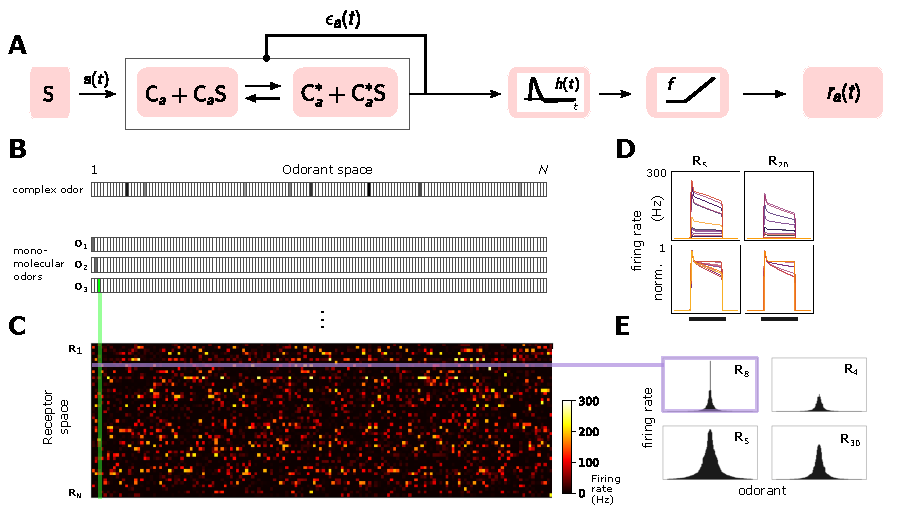
\includegraphics[width=\linewidth]{figures/1_tuning_curves}
	\caption{\footnotesize{
		\textbf{A}~Odor binding model. Or/Orco complexes $\textup{C}_a$ bind odorant molecules $s_i$ comprising stimuli $\textup{S}$. These complexes can stochastically switch between inactive and active states, where the steady-state active fraction is determined by the complex free energy $\epsilon_a(t)$. The activity feeds back on to the free energies with timescale $\tau$ to pull the activity to a baseline level $A_{a0}$. ORN firing rates $r_a(t)$ are generated by passing $A_a(t)$ through a linear temporal filter $h(t)$ and a nonlinear thresholding function$f$. 
		\textbf{B}~Odor mixtures are represented by real-valued $N$-dimensional vectors $\mathbf s$, whose components $s_i$ are the concentrations of  the individual molecular constituents  of $\mathbf s$. 
		\textbf{C}~Active binding constants are distributed as a power-law with coefficient $\alpha=0.35$~\cite{si2017invariances}.
		\textbf{D}~The maximal firing response of 50 ORNs to the 150-possible monomolecular odors $\mathbf s = s_i$, for the power-law $K^*_{ai}$ distribution in C.
		\textbf{E}~Representative ORN tuning curves, generated by ordering the responses within a single row of the response matrix in D. A diversity of response, mimicking that of~\cite{hallem_carlson}, arises from both the distribution of odorant binding constants $K^*_{ai}$ and the distribution of receptor free energies $\epsilon_a$.}}
		\label{fig:tuning_curves}
\end{figure*}

While in a single channel system such as \textit{E. coli} chemotaxis, adaptive feedback via Weber-Fechner's Law robustly maintains sensitivity over concentration changes~\cite{robustness_alon}, the implication for a multiple-channel system -- which combines information from several sensors with overlapping receptive fields  -- is less straightforward. Here we combine a biophysical model of universal ORN adaptive response and neural firing with various sparse signal decoding frameworks to explore how ORN adaptation affects combinatorial coding and decoding of odor signals spanning varying degrees of intensity, molecular complexity, and temporal structure. We find that this adaptive mechanism promotes the accurate  discrimination of weak odor signals from strong backgrounds of varying molecular complexity, both in static odor environments  and in fluctuating ones. We also investigate our framework in the context of the primacy coding hypothesis  -- that odors are encoded entirely by the few earliest responding ORNs~\cite{primacy_coding, primacy_math}, finding that primacy coding is both consistent with and enhanced by front-end adaptation. Together, our results suggest that despite the broad overlap of ORN tuning curves, a mechanism of front-end adaptation, when endowed with universal Weber-Fechner scaling via the co-receptor Orco, may play a vital role in preserving representations of odor identity in naturalistic odor landscapes.


\section*{Results}



%%%%%%%%%%%%%%%%%%%%%%%%%%%%%%%%%%%%%%%%%%%%%%%%%%%%%%%%%%%%%%%%%
%%%%%%%%%%%%    		MODEL DESCRIPTION    		%%%%%%%%%%%%%
%%%%%%%%%%%%%%%%%%%%%%%%%%%%%%%%%%%%%%%%%%%%%%%%%%%%%%%%%%%%%%%%%



\subsection*{Model of ORN sensing repertoire}

We consider a repertoire of $M=50$ ORN types modeled using a simple extension of a minimal model of odor-to-ORN firing~\cite{srinivas_elife} that reproduces the Weber-Fechner adaptation and firing rate dynamics measured in individual \textit{Drosophila} ORNs in response to Gaussian and naturalistic signals. Within ORNs of type $a=1,...,M$, Or-Orco complexes form non-selective cation channels (Fig.~\ref{fig:tuning_curves_a}) that stochastically switch between active and inactive states, while simultaneously binding to odorants $i$ with dissociation constants, $K^*_{ia}$ and $K_{ia}$, respectively~\cite{nagel_wilson_biophysical,srinivas_elife}. Assuming these processes are faster than other reactions in the signaling pathway, the quasi-steady state active fraction $A_a$ of channels in ORNs of type $a$ is (Methods):
\begin{align}
A_a(t) = \left(1 + e^{\epsilon_a(t)}\frac{1 + \sum_i^N s_i(t)/K_{ai}}{1 + \sum_i^N s_i(t)/K^*_{ai}}\right)^{-1}.
\label{eq:steady_state_act_OR}
\end{align}
$s_i(t)$ are the time-dependent concentrations of the individual monomolecular components of the odor signal $\bf{s}(t)$ at time $t$, and $N=150$ is the size of the molecular odorant space (Fig.~\ref{fig:tuning_curves_b}). Inward currents elicited by activating Or-Orco channels eventually result in a negative feedback onto $A_a(t)$~\cite{nagel_wilson_biophysical,srinivas_elife,cao_WL}:
\begin{align}
\tau\frac{d\epsilon_a(t)}{dt} = {A}_{a0} - A_a(t).
\label{eq:adaptation_dynamics}
\end{align}
Here $\tau$ is the adaptation time and $\epsilon_a(t)$ is the free energy change due to modifications of the Or-Orco complexes by the adaptation mechanism, which is  limited to the finite range $\epsilon_{\textup{L}, a} < \epsilon_a(t) < \epsilon_{\textup{H}, a}$~\cite{srinivas_elife}. Firing rate is minimally modeled by filtering the activity $A_a(t)$ with the double exponential filter $h(t)$ and rectifying nonlinearity $f$ (Methods and~\cite{srinivas_elife}):
\begin{align}
r_a(t)=f\left(h\otimes A_a(t)\right).
\label{eq:firing_machinery}
\end{align}
Here, $\otimes$ represents convolution. When deconvolved from stimulus dynamics, the shapes of the temporal kernels of \textit{Drosophila} ORNs that express Orco are largely receptor and odor independent~\cite{martelli,srinivas_elife,si2017invariances}. Moreover, adaptation is not intrinsic to the receptor~\cite{nagel_wilson_biophysical}. Accordingly, $\tau$, $h(t)$ and $f$ are assumed independent of receptor and odorant identities. 

We assume that the lower cutoffs $\epsilon_{\textup{L}, a}$ are receptor-dependent and choose them from a normal distribution. This variability ensures that ORNs are activated above quiescence (around 5 Hz) at distinct stimulus levels~\cite{srinivas_elife}. Diversity among odor-ORN responses mainly arises from the distribution of chemical dissociation constants. For simplicity we only consider agonists, i.e. $K^*_{ia}>K_{ia}$ but the analysis can easily be extended to include inhibitory odorants, which increases coding capacity~\cite{Cao_Tu_WL}. We choose the dissociation constants from a power law distribution ($\alpha = 0.35$) recently found across ORN-odor pairs in \textit{Drosophila} larvae (Fig.~\ref{fig:tuning_curves_c}). For a handful of ORNs we choose a very small value for one of the $K^*_{ai}$ to mimic high responders to private odorants relevant to innate responses. We checked that adding these private odors does not affect the general findings. 
 
While this phenomenological model could be extended to include further details -- e.g. we could relax the quasi-steady-state assumption in Eq.~\ref{eq:steady_state_act_OR} and use a more complex model for the firing rate~\cite{srinivas_elife} -- this minimally-parameterized form captures the key dynamical properties of Orco-expressing ORNs relevant to our study: receptor-independent adaptation~\cite{nagel_wilson_biophysical} with universal Weber-Fechner scaling~\cite{srinivas_elife,cafaro_WL,cao_WL,si2017invariances} that maintains response time independent of mean stimulus intensity~\cite{martelli,srinivas_elife}, and diversity of the tuning curves~\cite{hallem_carlson} and temporal firing patterns~\cite{stopfer_nat_neuro,stopfer_temporal_channel,stopfer_temporal_model} in response to panels of monomolecular odorants (Fig.~\ref{fig:tuning_curves_d}-\ref{fig:tuning_curves_e}). 




%%%%%%%%%%%%%%%%%%%%%%%%%%%%%%%%%%%%%%%%%%%%%%%%%%%%%%%%%%%%%%%%%
%%%%%%%%%%%%		CODING CAPACITY SECTION			%%%%%%%%%%%%%
%%%%%%%%%%%%%%%%%%%%%%%%%%%%%%%%%%%%%%%%%%%%%%%%%%%%%%%%%%%%%%%%%




\subsection*{Concentration-invariant preservation of coding capacity}% and abstract representations of odor identity}

\begin{figure}[!tb]
	\centering
	\begin{subfigure}[t]{\linewidth}
		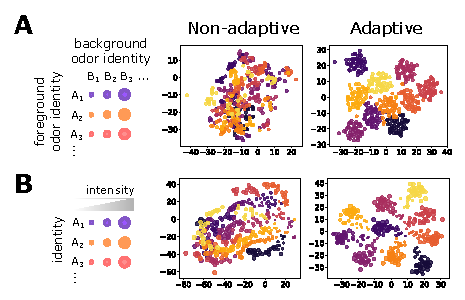
\includegraphics[width=\textwidth]{figures/2_coding_representation}
		\phantomsubcaption
		\label{fig:coding_a}
	\end{subfigure}
	\begin{subfigure}[t]{0\linewidth}
		\phantomsubcaption
		\label{fig:coding_b}
	\end{subfigure}
	\begin{subfigure}[t]{0\linewidth}
		\phantomsubcaption
		\label{fig:coding_c}
	\end{subfigure}
	\begin{subfigure}[t]{0\linewidth}
		\phantomsubcaption
		\label{fig:coding_3}
	\end{subfigure}
	\caption{\footnotesize{Front-end adaptation maintains information capacity and representations of odor identity across changes in intensity. 
		\textbf{A}~Step of odor A is followed by a step of odor B at a later time $t_B$, where $t_B \gg \tau$. Odor A and B have similar intensities.
    	\textbf{B}~Evolution of mutual information (MI) between odor signals and ORN response, in the non-adaptive system, as a function of relative odor concentration. Thin lines are the MI contained in individual ORNs; heavy line is the average. MI is plotted at times of order of $\tau$ following $t_A$ (purple; purple-blue), right before $t_B$ (blue-green), and shortly after $t_B$ (green).
		\textbf{C}~Same as (B), for the adaptive system.
		\textbf{D}~Abstract representation of ORN responses in reduced dimensions.
        }}
	\label{fig:coding}
\end{figure}

To investigate how front-end adaptation affects encoding capacity, we calculate the mutual information (MI) between odor signal $\mathbf s=\mathbf s_A +\mathbf s_B$ and response $\mathbf r$ as a function of signal intensity, with and without adaptation. A step of odor A, $\textbf{s}_A$,  turns on at time~$t_A$ and a step of odor B, $\mathbf s_B$ turns on at some later time~$t_B$ (Fig.~\ref{fig:coding_a}). Both odors have similar intensities. In the non-adaptive case, MI peaks around the region of maximum sensitivity ($\sim 10^2$ a.u.) after $t_A$ (Fig.~\ref{fig:coding_b}). The adaptive system mimics the non-adaptive system at $t_A$,  before adaptation has kicked in (Fig.~\ref{fig:coding_c}). In time, adaptation causes the sensitivity to decrease, %As the activity feeds back onto $\epsilon_a$, 
and the mutual information peak shifts to higher concentrations. Eventually, all ORNS are firing at adapted baseline and mutual information is mostly eliminated. However, having now adjusted its regime of maximum sensitivity to the presence of odor A, the system can respond appropriately to odor B: the MI at $t_B$ is nearly 6 bits across 3 decades of concentration.

We expect that preservation of information capacity helps maintain  odor identity. We visualize this by projecting the 50-dimensional ORN  response $\mathbf r$ to a lower two-dimensional space using t-distributed stochastic neighbor embedding (t-SNE)~\cite{tsne}. Testing this both for a smaller (Fig.~\ref{fig:coding_d}) and larger (Supporting Information) odor repertoire, odors cluster by identity in the adaptive system, while in the non-adaptive system, representations  mix among their identity and concentration. This suggests that universal front-end adaptative feedback helps preserves odor identities within the ensemble of ORN response.

%%%%%%%%%%%%%%%%%%%%%%%%%%%%%%%%%%%%%%%%%%%%%%%%%%%%%%%%%%%%%%%%%
%%%%%%%%%%%%    		SIGNAL DECODING      	     %%%%%%%%%%%%
%%%%%%%%%%%%%%%%%%%%%%%%%%%%%%%%%%%%%%%%%%%%%%%%%%%%%%%%%%%%%%%%%




\begin{figure*}[t]
	\centering
	\begin{subfigure}[t]{17.7cm}
		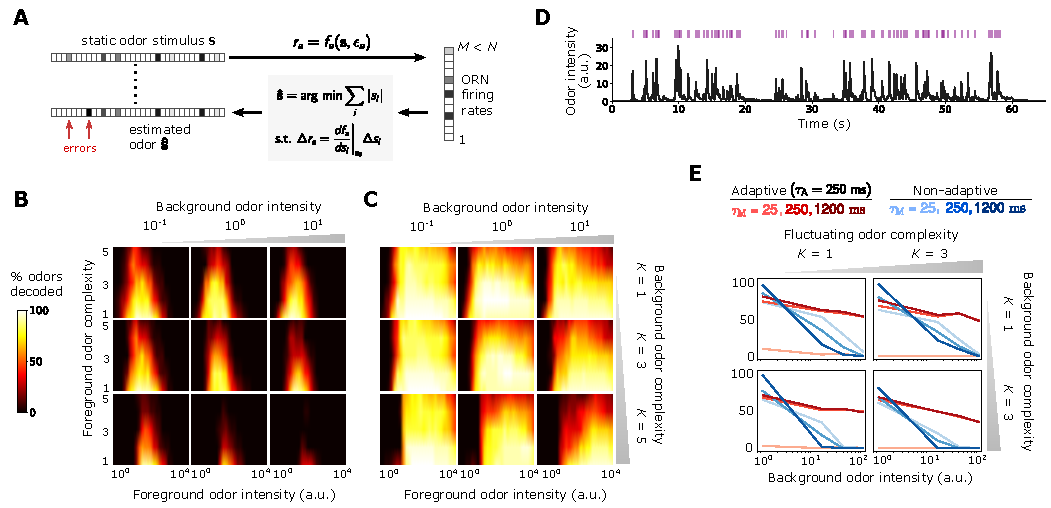
\includegraphics[width=17.7cm]{figures/3_decoding_temporal}
		\phantomsubcaption
		\label{fig:decoding_a}
	\end{subfigure}
	\begin{subfigure}[t]{0\linewidth}
		\phantomsubcaption
		\label{fig:decoding_b}
	\end{subfigure}
	\begin{subfigure}[t]{0\linewidth}
		\phantomsubcaption
		\label{fig:decoding_c}
	\end{subfigure}
	\begin{subfigure}[t]{0\linewidth}
		\phantomsubcaption
		\label{fig:decoding_d}
	\end{subfigure}
	\begin{subfigure}[t]{0\linewidth}
		\phantomsubcaption
		\label{fig:decoding_e}
	\end{subfigure}
	\caption{\footnotesize{Front-end adaptation promotes accurate sparse odor decoding in static and naturalistic odor environments.
    \textbf{A}~Odor stimuli produce ORN responses via odor-binding and activation and firing machinery, as described by Eqs.~\ref{eq:steady_state_act_OR}-\ref{eq:firing_machinery}. Odors are then decoded using compressed sensing by linearizing around a background $s_0$ and minimizing the constrained $L_1$ norm of the odor signal (Methods).  Odors are assumed sparse, exhibiting $K$ nonzero components, $K \ll N$. 
    \textbf{B}~Decoding accuracy of foreground odors in the presence of background odors, without front-end adaptation. Individual heatmaps show the decoding accuracy of the foreground odor as a function of its intensity and complexity; plots are arrayed by background odor intensity (column-wise) and complexity (row-wise). Odors are considered accurately decoded if the sparse components are estimated within 25\% of their true values and the zero components (not in the odor mixture) are estimated below 10\% of $s_0$.
    \textbf{C}~Same as (B), for the adaptive system.
    \textbf{D}~Recorded trace of naturalistic odor signal; whiffs (signal > 5 a.u.) demarcated by purple bars. This signal is added to static backgrounds of different intensities and complexities, which is then decoded in time (Methods).
    \textbf{E}~Individual plots show the percent of accurately decoded odor whiffs as a function of background odor intensity, for the non-adaptive (blue) and adaptive (red) systems, for different $t_{\textup F}$ (line shades). Plots are arrayed by the complexity of the naturalistic signal (column-wise) and the complexity of the background odor (row-wise)
    }}
	\label{fig:decoding}
\end{figure*}


\subsection*{Front-end adaptation enhances odor discrimination in complex environments}

How well does the preservation of coding capacity translate to better signal reconstruction?
%Next, we ask how the universal adaptive feedback might contribute to accurate signal reconstruction from ORN responses. 
One potentially complicating factor is the disparity between sensor dimension and stimulus dimension: while \textit{Drosophila} only express $\sim 60$ olfactory receptor genes~\cite{olfactory_sensory_map}, the space of odorants is far greater~\cite{vijay_1}. However, many naturally-occurring odors are comprised of a small subset of odorants, which is suggestive as mathematical results in compressed sensing guarantee their reconstruction, assuming a sufficiently random response~\cite{vijay_1, CS_donoho, CS_tao, CS_ganguli}. There is no direct evidence that a compressed decoding framework is implemented in the \textit{Drosophila} olfactory circuit~\cite{chlovskii_pevlavan}. Here we used this framework as a mathematical tool to quantify how front-end adaptation potentially affects odor decoding. We later verify our conclusions with other classification techniques that make use of the known architecture of the olfactory system. 

To incorporate the linear framework of compressed sensing, we treat the nonlinear odor encoding exactly but approximate the decoding to first order. We first examine how foreground odors are recognized when mixed with background odors, quantifying decoding accuracy as the percentage of odors correctly decoded within some tolerance (Methods; Fig.~\ref{fig:decoding_a}). Without adaptation, detection accuracy for concentrations is maintained within the range of receptor sensitivity, for a simple, weak background. However, accuracy is virtually eliminated as background complexity and intensity rise (Fig.~\ref{fig:decoding_b}). The range of the sensitivity is higher in the adaptive system, and it is substantially more robust across changes in molecular complexity and intensity of the background odors (Fig.~\ref{fig:decoding_c}). 

In realistic odor environments, the concentration and duration of individual odor whiffs vary widely~\cite{celani}, and we wondered how well a front-end adaptation mechanism with a single timescale $\tau$ could promote whiff detection in such environments. As inputs to our coding/decoding framework we apply a naturalistic stimulus intensity recorded using a photo-ionization detector~\cite{srinivas_elife} (Fig.~\ref{fig:decoding_d}) to which we randomly assign sparse identities from the $N$-dimensional odorant space. To mimic background confounds, we combine these signals with static odor backgrounds, and then calculate the percentage of decoded whiffs (purple bars in Fig.~\ref{fig:decoding_d}). We also assume a finite length of short-term memory: detected odor signals are only retained $\tau_{\textup {F}}$ seconds in the immediate past (Methods). Without ORN adaptation, sufficiently strong backgrounds eliminate the ability to reconstruct the identity of individual odor whiffs, irrespective of the complexity of either the foreground or background odor (Fig.~\ref{fig:decoding_e}, green lines). In the adaptive system, this is substantially mitigated (red lines in Fig.~\ref{fig:decoding_e}), as long as the memory duration $\tau_{\textup {F}}$ is on the same order as the adaptation timescale $\tau$ (darker red lines). %Thus, we find that universal front-end adaptation with a single timescale promotes detection of naturalistic odor signals amidst confounding backgrounds of varying complexity and intensity.





\subsection*{Front-end adaptation enhances primacy coding}

The primacy coding hypothesis posits that odor identity is encoded by the set (but not temporal order) of the $p$ earliest responding glomeruli/ORN types, known as primacy set of order $p$~\cite{primacy_coding}. If the activation order of ORNs were invariant to the strength of an odor step or pulse, primacy sets would in principle form concentration-invariant representation of odor identity. 

Though our coding framework uses the full ORN ensemble in signal reconstruction, some of these ORN responses may contain redundant information, and a smaller primacy subset may suffice. To examine this relationship, we apply our model to a sigmoidal stimulus that rises to half-max in 50 ms, calculating decoding accuracy in time. Since ORNs activate sequentially, the primacy set is defined by the ORN subset active when the odor is accurately decoded. For simple odors, a limited set of earliest responding neurons fully accounts for the odor identity ($K=1, 3, 5$ plots in Fig.~\ref{fig:primacy_coding_a}), in agreement with primacy coding. %Though all ORNs eventually activate as the stimulus increases, the latter responders confer no further information in odor recognition. 
As expected for more complex odor mixtures, the full repertoire is required for accurate decoding ($K=7, 9$ plots in Fig.~\ref{fig:primacy_coding_a}). Primacy coding also predicts that for stronger stimuli, responses occur earlier in time, since the primacy set is realized quicker, which our framework replicates (SI).

Beyond mere consistency, however, front-end adaptation might also enhance primacy coding in different environmental conditions, such as background odors, which could scramble primacy sets. %Might front-end adaptation help maintain primacy sets in the presence of environmental confounds, such as background odors? %Having adapted to a background, an ORN could in principle be pushed out of the primacy set of a novel odor, due to its reduced sensitivity. 
To investigate this, we calculated the primacy sets for 1000 sparse odor mixtures atop various static backgrounds. We find that primacy sets for these mixtures are preserved across different background concentrations, for all but the smallest primacy orders (Fig.~\ref{fig:primacy_coding_c}). This suggests that front-end adaptation may play a central role in reinforcing primacy codes across differing environmental conditions. 


\subsection*{Contribution of front-end adaptation for odor recognition within the \textit{Drosophila} olfactory circuit}


\begin{figure}[tb]
	\begin{subfigure}[t]{\linewidth}
		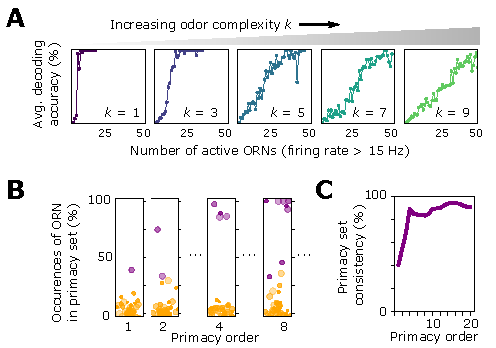
\includegraphics[width=\textwidth]{figures/4_primacy_coding}
		\phantomsubcaption
		\label{fig:primacy_coding_a}	
	\end{subfigure}
	\begin{subfigure}[t]{0\linewidth}
		\phantomsubcaption
		\label{fig:primacy_coding_b}
	\end{subfigure}
	\begin{subfigure}[t]{0\linewidth}
		\phantomsubcaption
		\label{fig:primacy_coding_c}
	\end{subfigure}
	\caption{\footnotesize{
	\textbf{A} Decoding accuracy as a function of the number of active ORNs (firing rate~$>$~15 Hz), for different odor complexities. The primacy set consists of those ORNs required to be active for accurate decoding; the set size grows with odor complexity.
	\textbf{B} Number of active ORNs required to fully decode odor signals of varying odor intensity and complexity. 
	\textbf{C} Primacy sets for a step signal in the presence of different background intensities are almost identical for all but the smallest primacy orders  ($p \gtrapprox 5$). Yellow: overlap of the primacy sets for step signal when placed atop a weak (1x) vs. a medium (10x) background; purple: overlap of primacy sets for step signal atop weak vs. strong (100x) backgrounds.
	}}
	\label{fig:primacy_coding}
\end{figure}

Signal transformations in the sensing periphery are propagated through the remainder of the olfactory circuit, where they are ultimately translated to behavioral response. How does front-end adaptation interact with these subsequent neural transformations? ORNs expressing the same OR converge to a unique AL glomerulus, where they receive lateral inhibition from other glomeruli~\cite{lateral_inh, lateral_inh_asahina}. This inhibition implements a type of divisive gain control~\cite{divisive_normalization}, normalizing the activity of output projections neurons, which then synapse onto a large number of Kenyon cells (KCs) in the mushroom body. %. The circuit diverges collective responses are normalized through divisive normalization. Outputs from these 60 glomeruli then diverge, connecting synaptically onto Lateral inhibition among antennal lobe (AL) glomeruli normalizes ORN responses prior to their projections to the mushroom body by implementing a type of divisive gain control. 
To investigate how odor representations are affected by interactions between front-end ORN adaptation and this lateral inhibition and synaptic divergence, we extended our ORN encoding model by adding uniglomerular connections from ORNs to the antennal lobe, followed by sparse, divergent connections to 2500 KCs~\cite{memory_review, litwinkumar, abbott_axel}. Inhibition was modeled via divisive normalization, with parameters chosen according to experiment~\cite{divisive_normalization}.
%\begin{align}
%r_{\textup{PN}, a}(t) = \frac{r_a(t)^{1.5}}{\sigma^{1.5} + r_a(t)^{1.5} + (\gamma\sum_b^Mr_b(t))^{1.5}}
%\end{align}
We quantified decoding accuracy by training and testing a binary classifier on the KC activity output of sparse odors of distinct intensity and identity, randomly categorized as appetitive or aversive. Odor signals of the same identity but differing intensity were assigned the same valence. We trained the classifier on $N_{\text ID}$ sparse odor identities at intensities chosen randomly over 4 orders of magnitude, then tested the classifier accuracy on the same odor identities but of differing concentrations. 

Classification accuracy degrades to chance level as $N_{\text ID}$ becomes very large (Fig.~\ref{fig:downstream_a}). When acting alone, either divisive normalization or ORN adaptation can help, although the effect of ORN adaptation is stronger. When both are active, accuracy improves further, suggesting that these distinct adaptive transformations may act jointly at different stages of neural processing in preserving representations of odor identity. Interestingly, if we train the classifier to distinguish odors by their distinct identity, rather than valence, we find that the benefits conferred by divisive normalization do not appear until $N_{\text ID}$ is substantial, with accuracy below $65\%$ for $N_{\text ID} > 50$ (Fig.~\ref{fig:downstream_b}). On the other hand, with ORN adaptation accuracy remains above $85\%$ for more than 1000 odor identities, strongly implicating front-end adaptation as a key player in maintaining odor identity representations, before they are further processed downstream. 


%{\color{blue} Code with temporal sequence of odors, not strength or subset? Each vector is  the sequence of temporal activation -- does adaptation help? }









%%%%%%%%%%%%%%%%%%%%%%%%%%%%%%%%%%%%%%%%%%%%%%%%%%%%%%%%%%%%%%%%%
%%%%%%%%%%%%	   	        DISCUSSION                %%%%%%%%%%%
%%%%%%%%%%%%%%%%%%%%%%%%%%%%%%%%%%%%%%%%%%%%%%%%%%%%%%%%%%%%%%%%%





\section*{Discussion}

%{\color {blue}-- also don't forget to mention that the odor-receptor  interactions are nonlinear and that saturation is important in this case -- also many odors  Stopfer -- information in each pulse enough (small 50s bins) is enough to classify odors . Go further here and say that even in odor connfounds and complex odors, same conclusion follows. maybe do this for temporal presentation, not odor reconstruction, just order?}


We investigate the theoretical implications of observed universal input gain control in \textit{Drosophila} olfactory receptor neurons. We argue that such gain control, obeying the Weber-Fechner Law of psychophysics, plays a central role in preserving neural representations of odor identity at the front-end of the olfactory pathway. Our conclusions rely on both a compressed sensing scheme that fully reconstructs odor signals from neural response, as well as classification algorithms that categorize odors by identity or valence. We find that input gain control acting on a single timescale of $\sim 250$ ms enhances the coding capacity of ensemble ORN response, helping maintain representations of odor identity independent of intensity (Figs.~\ref{fig:tuning_curves} and  \ref{fig:coding}). %It allows robust determination of odor identity from single whiffs when mixed among static backgrounds, and 
%. Increases in the strength and complexity of background odors rapidly scramble odor codes in non-adaptive systems, a degradation that is substantially mitigated with the addition of ORN adaptation.
It acts jointly with normalization in the antennal lobe to aid the discrimination of naturalistic, dynamic odor signals from static backgrounds, implicating the importance of signal transformations at multiple steps in the olfactory circuit (Figs.~\ref{fig:decoding} and \ref{fig:downstream}). We also study our model in the context of primacy coding -- that signals are encoded by the earliest activating glomeruli -- finding that front-end adaptation enhances primacy coding by maintaining primacy sets amid background confounds (Fig.~\ref{fig:primacy_coding}).

\begin{figure}[tbh]
	\centering
	\begin{subfigure}[t]{\linewidth}
		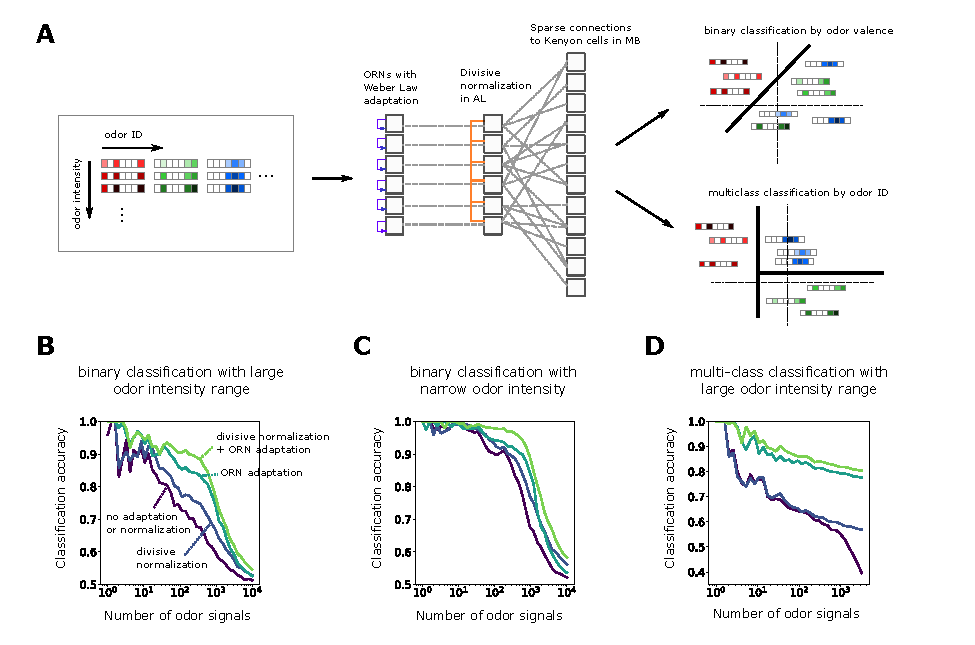
\includegraphics[width=\textwidth]{figures/5_downstream}
		\phantomsubcaption
		\label{fig:downstream_a}	
	\end{subfigure}
	\begin{subfigure}[t]{0\linewidth}
		\phantomsubcaption
		\label{fig:downstream_b}
	\end{subfigure}
	\begin{subfigure}[t]{0\linewidth}
		\phantomsubcaption
		\label{fig:downstream_c}
	\end{subfigure}
	\begin{subfigure}[t]{0\linewidth}
		\phantomsubcaption
		\label{fig:downstream_d}
	\end{subfigure}
	\caption{\footnotesize{
	\textbf{A} Accuracy of binary classification by odor valence, as a function of the number of distinct odor identities classified by the trained network (concentrations span 4 orders of magnitude), in systems with only ORN adaptation, only divisive normalization, both or neither. \textbf{B} Same as (A) but now classifying odors  by identity.
	}}
	\label{fig:downstream}
\end{figure}

LIMITATIONS OF THIS WORK \\
LIMITATIONS OF THIS WORK \\
LIMITATIONS OF THIS WORK \\
LIMITATIONS OF THIS WORK \\
LIMITATIONS OF THIS WORK \\
LIMITATIONS OF THIS WORK \\


%Our results are relevant for understanding combinatorial odor coding in naturalistic odor environments. %As ORN adaptation can be decoupled from neural firing using optogenetic stimulation~\cite{srinivas_elife}, these results could be tested in behavioral assays that 
%It is notable that both Weber-Fechner adaptation and divisive normalization modulate the location of maximal sensitivity rather than the scale of absolute activity -- they move dose-response curves horizontally, rather than stretching them vertically. They are both mechanisms of input gain control rather than response gain control. {\color{blue} Such input mechanisms are common to other models, sensory ssytems, etc... (...la)}. 



Previous studies in the \textit{Drosophila} olfactory circuit have characterized the impact of various response characteristics in maintaining combinatorial codes. Lateral inhibition helps tame saturation and boost weak signals~\cite{divisive_normalization}. ORNs exhibiting both excitatory and inhibitory responses to odorants can increase coding capacity by exploiting response bidirectionality~\cite{Cao_Tu_WL}. In vertebrates, G-protein-coupled chemoreceptors rather than Orco-coupled cation channels, antagonism among odorants may help maintain response sparsity~\cite{reddy2017antagonism}. Finally, in both vertebrates and insects, the degree of connectivity to either the olfactory bulb or mushroom body (each KC receives connections from only $\sim$6 AL glomeruli) may be precisely tuned to optimize the system's capacity to learn associations~\cite{litwinkumar}. Our results show that a number of these downstream features are enhanced front-end dynamic adaptation. 

Other studies in insect olfaction have implicated the unique temporal patterns of neural response as signatures of odor identity~\cite{stopfer_temporal_model, multiple_timescales_stopfer, stopfer_nat_neuro, stopfer_temporal_channel}. ORN and projection neuron time traces form distinct trajectories in low-dimensional projections, and cluster by odor identity, much as we have found here (Fig.~\ref{fig:coding_b}). %Though we do explicitly utilize the temporal history of neural firing in our decoding schemes, the transmission of information over time is implicit in this framework. 
In our framework, temporal coding is implicit. Because the strength of ORN feedback onto receptor complex activation depends on an ORN's unique response characteristics, odor signals are naturally formatted into temporal patterns that are both odor- and ORN-specific --  despite the universality of~$\tau$. Further, the short forgetting timescales, $\tau_{\textup F} \sim \tau \sim 250$ ms, suggest that only brief time windows are needed for accurate odor identification, consistent with previous findings~\cite{stopfer_nat_neuro}. 

In living systems, sensory adaptation ensures that responses remain in regimes of maximum sensitivity, increasing their effective dynamic range~\cite{adaptation_fairhall, adaptation_nagel, laughlin, deweese_adaptation}. Doing so requires matching sensory response to attributes of the environment, either by adapting to specific stimuli or to stimuli statistics~\cite{adaptation_fairhall}. 
%Viewing sensory systems as input/output machines, the role of adaptation is therefore to maintain information capacity in dynamic environments~\cite{information_theory_adaptation}. 
In a single-channel system such as bacterial chemotaxis, information capacity is increased by matching the midpoint of the nonlinear dose-response curve, where sensitivity is highest, to mean ligand concentration~\cite{information_theory_adaptation}. This is enacted in a robust and dynamic way, through a feedback loop from the activity output of the pathway onto proteins dictating receptor sensitivity~\cite{robustness_barkai, robustness_alon}. We hypothesize that an analogous feedback loop exists in olfactory receptor neurons, from Orco-mediated Or channel activity onto the free energy of receptor activation~\cite{srinivas_elife}. %Orco  itself consists of four subunits arranged symmetrically around a central pore, with two of the sub-units possibly conferring odor specificity~\cite{orco_structure}. If 
This mechanism appears to act identically across ORNs, and because olfactory tuning curves are highly overlapping, raises questions about its efficacy in complex environments: adaptation to one odor could adversely affect identification of a new odor if the latter excites some but not all of the same ORNs. Our results show that this general feedback, operating at a single timescale, does help to preserve combinatorial representations of odor identity, despite these broad overlaps. 



%%%%%%%%%%%%%%%%%%%%%%%%%%%%%%%%%%%%%%%%%%%%%%%%%%%%%%%%%%%%%%%%%
%%%%%%%%%%%%	   	           METHODS                %%%%%%%%%%%
%%%%%%%%%%%%%%%%%%%%%%%%%%%%%%%%%%%%%%%%%%%%%%%%%%%%%%%%%%%%%%%%%




\section*{Methods}

\iffalse
{\color {blue} This section needs to be redone}
\subsection*{Odor-receptor binding model}

We model an odor as an $N$-dimensional vector ${\mathbf s=[ s_1,...,s_N]}$, where $s_i > 0$ are the concentrations of individual volatile molecules (odorants) comprising the odor. 
The olfactory sensory system is modeled as a collection of $M$ distinct Or/Orco complexes, each of which can be bound with any one of the odorant molecules, and can be either active (firing) inactive (quiescent). We only consider competitive binding, so a complex is bound with one odorant at most. With $N$ possible odorants, receptor $a$ resides in one of $2N+2$ possible states, \{$R_a$, $R^*_a$, $R_a$-$s_i$, $R^*_a$-$s_i$\}, indicating receptors that are unbound/inactive, unbound/active, inactive/bound to odorant $i$, and active/bound to odorant $i$, respectively. We set $N = 150$ and $M = 50$ throughout.

In the mean-field limit, the binding dynamics of these $2N + 2$ states are described by the master equations:

\begin{align}
\frac{d[R_a\text{-}s_i]}{dt} &= k^+_{ia}s_i[R_a] - k^-_{ia}[R_a\text{-}s_i] \label{eq:Meq_inactive_bind_rate}\\
\frac{d[R^*_a\text{-}s_i]}{dt} &= k^{*+}_{ia}s_i[R^*_a] - k^{*-}_{ia}[R^*_a\text{-}s_i],
\label{eq:Meq_active_bind_rate}
\end{align}
when receptor $R_a$ is either inactive (Eq.~\ref{eq:Meq_inactive_bind_rate}) or active (Eq.~\ref{eq:Meq_active_bind_rate}). Further, transitions between inactive and active states are described in the mean limit via:
\begin{align}
\frac{d[R_a]}{dt} &= w^{\text{u}+}_a [R_a] - w^{\text{u}-}_a [R^*_a] \label{eq:Meq_unbound_active_rate}\\
\frac{d[R^*_a\text{-}s_i]}{dt} &=  w^{\text{b}+}_{ia} [R_a\text{-}s_i] - w^{\text{b}-}_{ia}  [R^*_a\text{-}s_i],
\label{eq:Meq_bound_active_rate}
\end{align}
when receptor $R_a$ is either unbound (Eq.~\ref{eq:Meq_unbound_active_rate}) or bound (Eq.~\ref{eq:Meq_bound_active_rate}). The corresponding disassociation constants in terms of the binding transition rates are:


\begin{align}
K_{ai} = \frac{k^-_{ai}}{k^+_{ai}} \nonumber \\
K^*_{ai} = \frac{k^{*-}_{ai}}{k^{+*}_{ai}} 
\label{eq:Kd}
\end{align}

Following~\cite{srinivas_elife}, we assume that in steady state, the active firing state of an Or/Orco complex is energetically suppressed from the inactive state through corresponding Boltzmann factors:

\begin{align}
\frac{[R^*_a]}{[R_a]} &= \frac{w^{\text{u}+}_a}{w^{\text{u}-}_a} \equiv e^{-\epsilon_a} \label{eq:epsilon_unbound} \\
\frac{[R^*_a\text{-}s_i]}{[R_a\text{-}s_i]} &= \frac{w^{\text{b}+}_{ia}}{w^{\text{b}-}_{ia}} \equiv e^{-\epsilon^{\text b}_{ia}}.\label{eq:epsilon_bound}
\end{align}
These energies are related through detailed balance, which we assume. Applying detailed balance to a given 4-cycle 
\begin{align}
R_a \rightarrow R_a^* \rightarrow R_a^*\text{-}s_i \rightarrow R_a\text{-}s_i \rightarrow R_a
\end{align}
gives
\begin{align}
\frac{w^{\text{u}+}_a}{w^{\text{u}-}_a}\frac{k^{*+}_{ia}}{k^{*-}_{ia}}\frac{w^{\text{b}-}_{ia}}{w^{\text{b}+}_{ia}}\frac{k^{-}_{ia}}{k^{+}_{ia}} \equiv 1,
\label{eq:detailed_balance}
\end{align}
which, in conjunction with Eqs.~\ref{eq:Kd}, \ref{eq:epsilon_unbound}, and \ref{eq:epsilon_bound}, gives
\begin{align}
\epsilon_{ai}^{\text b} = \epsilon_{a, \textup{act}} + \ln\left[\frac{K^*_{ai}}{K_{ai}}\right].
\label{testing_equation}
\end{align}
Assuming the binding dynamics are fast, then the probability that receptor $a$ is bound by ligand~$i$ when inactive and active can be derived from  Eqs.~\ref{eq:Meq_inactive_bind_rate} and \ref{eq:Meq_active_bind_rate} as
\begin{align}
p^{\text b}_{ai} = \frac{s_i/K_{ai}}{1 + \sum_j^Ns_j/K_{aj}} \label{eq:bound_prob_ai_inactive} \\
p^{\text b, *}_{ai} = \frac{s_i/K^*_{ai}}{1 + \sum_j^Ns_j/K^*_{aj}} \label{eq:bound_prob_ai_active}.
\end{align}
The average  activity $A_a$ of complex $a$ is the likelihood that the complex is active, unbound or unbound (equivalantly, the proportion of Or/Orco complexes in a given ORN that are active):
\begin{align}
A_a = \frac{[R^*_a] + \sum_i^N[R^*_a\text{-}s_i]}{[R^*_a] + \sum_i^N[R^*_a\text{-}s_i] + {[R_a] + \sum_i^N[R_a\text{-}s_i]}}.
\end{align} 
Using the master equations between active and inactive states Eq.~\ref{eq:Meq_unbound_active_rate} and \ref{eq:Meq_bound_active_rate}, $A_a$  obeys the master equation
\begin{align}
\frac{dA_a}{dt} &= w^+_a(1 - A_a) + w^-_aA_a
\label{eq:dadt}
\end{align}
with effective transition rates
\begin{align}
w^+_a &= \sum_i^Np^{\text b}_{ai} w^{\text u +}_{ai} + p_{a}w^{\text u}_a 
\end{align}
and analogously for $w_a^-$. Setting Eq.~\ref{eq:dadt} to zero gives the steady state average activity level of Or/Orco complex $a$:
\begin{align}
A_a = \left(1 + e^{\epsilon_{a, \textup{act}}}\frac{1 + \sum_i^N s_i/K_{ai}}{1 + \sum_i^N s_i/K^*_{ai}}\right)^{-1}. \tag{\ref{eq:steady_state_act_OR}}
\end{align}
	
\subsection*{ORN firing response}

Receptor activity $A_a$ is a measure of cation influx into ORNs elevates the ORN membrane voltage, which can then incite a sustained firing response. A faithful representation of this process would require a Hodgkin-Huxley-type model. These dynamics can be largely captured by a linear-nonlinear response, which we adopt here. 

\subsection*{Generation of binding matrices $K^*_{ia}$}
 TODO

\subsection*{Compressed sensing decoding of ORN response}
We decode ORN responses to infer odor signal identities using an abstraction intended to mimic the neural computations underlying odor identification in the \textit{Drosophila} mushroom body. While we make no assumptions that the compressed sensing (CS) algorithm (or one like it) is being utilized in actuality, this framework nonetheless informs our understanding of how the neural representation of odor identity is maintained or lost when passed through a distributed ORN repertoire. In this sense, CS is somewhat of an upper bound on how well a real neural computation might perform in decompressing ORN responses.

We assume that ORN firing rates are linear in the Or/Orco complex activity; for simplicity we let this transform be the identity. Though subsequent neural circuitry, particularly from the glomeruli in the AL to the Kenyon cells in the MB further mix and scramble these responses, we focus here on the information transfer at the sensory periphery alone. In any case, as demonstrated previously~\cite{vijay_1}, we expect that these neural computations would only improve the representation of neural identity, so we expect no negative ramifications for our findings.

CS addresses the problem of determining a sparse signal from a set of linear measurements, when the number of measurements is less than the signal dimension. Specifically, it is a solution to 
\begin{align}
\mathbf y = \mathbf R\mathbf s,
\label{eq:CS_constraints}
\end{align} where $\mathbf s \in \mathbb{R}^N$ and $\mathbf a\in \mathbb{R}^M$ are vectors of signals and responses, respectively, and $\mathbf R$ is the measurement matrix. Since measurements are fewer than signal components, then $M < N$, whereby $\mathbf R$ is wide rectangular and so Eq.~\ref{eq:CS_constraints} cannot be simply inverted to produce $\mathbf s$. The idea of CS is to utilize the knowledge that $\mathbf s$ is sparse, i.e.g only $K$ of its components, $K \ll N$ are nonzero. Both the measurements and sparsity are thus combined into a single constrained optimization routine:
\begin{align}
\hat s_i = \textup{argmin} \sum_i^N |s_i| \quad \textup{such that } \mathbf y = \mathbf R\mathbf s
\label{eq:CS}
\end{align}
where $\hat s_i$ are the optimal estimates of the signal components and the sum, which is known as the $L_1$ norm of $\mathbf s$, is a natural metric of sparsity. 

Importantly, the $L_1$ norm is a convex operation and the constraints are linear, so the optimization has a unique global minimum. To incorporate the nonlinear response of our encoding model into this linear framework, we assume that the responses are generated through the full nonlinear steady state response, Eq.~\ref{eq:steady_state_act}, but that the measurement matrix needed for decoding uses a linear approximation of this transformation.  Expanding Eq.~\ref{eq:steady_state_act} around $s_0 = s_i - \Delta s_i$ gives
\begin{align}
A_a &\approx A_{a, 0} + \Delta A_a \label{eq:CS_act_approx} \\
\Delta A_a &= \sum_i^NR_{ia}\big|_{s_0}\Delta s_i \label{eq:CS_dAct_approx}\\
A_{a, 0} &= \frac{\sum_1^N s_0/K_{ia}^*}{\sum_1^N s_0/K_{ia}^* + e^{\epsilon_a}} \label{eq:CS_act0_approx} \\
R_{ia}\big|_{s_0} &=  \frac{e^{\epsilon_a}/K_{ia}^*}{(\sum_i^Ns_0/K_{ia}^* + e^{\epsilon_a})^2},
\label{eq:CS_gain_approx}
\end{align}
where we work in the approximation $K^*_{ia} \ll~s_0 \ll K_{ia}$. We assume that the neural system has access to the linearized response, Eq.~\ref{eq:CS_gain_approx}, but must infer the excess signals $\Delta s_i$ from the excess activity $\Delta A_a$. Corresponding to the CS framework, therefore, $\Delta \mathbf {A} \rightarrow \mathbf y$, $\Delta \mathbf s \rightarrow \mathbf s$, and $R_{ia}\big|_{s_0} \rightarrow \mathbf R$. We optimize the cost function in Eq.~\ref{eq:CS} using sequential least squares programming, implemented in Python through using the scientific package SciPy.

\subsection*{Or/Orco  energies of activation $\epsilon_a$ and enforcement of Weber's Law}
Free energies are considered receptor-independent throughout, with the exception of dynamically adaptive system in a temporal odor environment (Figs.~\ref{fig:temporal_coding} and \ref{fig:temporal_coding_2}). To enforce Weber's Law, we assume the receptor activities feed back onto $\epsilon_a$ through the free energies. For the static case, adaptation is perfect, whereby Or/Orco activities are pegged to perfectly adapted values $\bar {A}_{a}$. Incorporating this into Eq.~\ref{eq:steady_state_act}, and assuming  $K^*_{ia} \ll s \ll K_{ia}$, gives
\begin{align}
\bar \epsilon_a &= \ln\left(\frac{1-\bar {A}_{a}}{\bar {A}_{a}}\right) + \ln\left(\sum_i^N\frac{s_i}{K_{ia}^*}\right).
\label{eq:adapted_epsilon}
\end{align}
Assuming that the excess signals are small, $\Delta s_i < s_0$, this gives 
\begin{align}
\epsilon_a \approx \ln(s_0) + \epsilon_{a, 0},
\label{eq:WL_approx}
\end{align} 
where $\epsilon_{a, 0}$ are receptor-dependent constants. In the static case, we choose these constants such that $\epsilon_{a}$ in both adaptive and non-adaptive systems are equivalent, equal to $\epsilon_{\text {L}}$, at a given low concentration, $s_{0, \text L}$.  Below this concentration, we assume adaptation is not in effect, so $\epsilon_a  = \epsilon_{\text {L}}$.  

It is important to note that while the linearized gain Eq.~\ref{eq:CS_gain_approx} utilized by the decoding algorithm appears to rely on $\epsilon_a$, by the above argument $\epsilon_a$ can in principle be determined by firing rates alone. That is, $\epsilon_a$ is inferred in time through integration of Eq.~\ref{eq:WL_dynamics}, which relies only on the current ORN activity.


\begin{table*}[!tb]
	\centering
	{\small
		\begin{tabular}{ccccccccccccccc}
			Figure & $N$& $M$ & $K$ & $\mu_{a, \text L}$ & $\mu_{a, \text H}$ & $\nu_{a, \text L}$ & $\nu_{a, \text H}$ & $\epsilon_{a, 0}$ & $\epsilon_{\text {L}}$  & $\epsilon_{\text {H}}$  & $s_{0, \text L}$ & $s_k$ & $s_{k, \text F}$\\[0.1cm]
			
			\hline \\[-0.2cm]
			\smallskip
			
			\ref{fig:tuning_curves_c} & 200 & 40 & 6 & $2\cdot 10^{-4}$ & $10^{-3}$ & $10^{-2}$ & 1.0 & 5.4 & 5.4 & 10  & - & $ \mathcal N\left(\frac{s_0}{5}, \frac{s_0}{15}\right)$ & --\\
			
			\ref{fig:decoding_a} & 100 & 50 & 7 & 0.5 & 0.5 & 0.8 & 0.8 & 5.4 & 3.1 & 10  & $10^{-1}$ & $ \mathcal N\left(\frac{s_0}{3}, \frac{s_0}{15}\right)$ & -- \\
			
			\ref{fig:decoding_b} & 100 & 50 & 7 & 0.5 & 0.6 & 0.6 & 0.9 & 5.4 & 3.1 & 10 & $10^{-1}$ & $ \mathcal N\left(\frac{s_0}{3}, \frac{s_0}{15}\right)$ & ---\\
			
			\ref{fig:decoding_c} & 100 & 50 & 7 & 0.5 & 0.6 & 0.6 & 0.9 & 5.4 & 3.1 & 10 & $10^{-1}$ & $ \mathcal N\left(\frac{s_0}{3}, \frac{s_0}{15}\right)$ & -- \\
			
			\ref{fig:signal_discrimination_a}-\ref{fig:signal_discrimination_h} & 100 & 50 & 7 & 0.5 & 0.6 & 0.6 & 0.9 & 5.4 & 3.1 & 10 & $10^{-1}$ & $ \mathcal N\left(\frac{s_0}{3}, \frac{s_0}{15}\right)$ & $ \mathcal N(1, \frac{1}{5})$ \\
			
			\ref{fig:temporal_coding} & 100 & 50 & 7 & 0.5 & 0.6 & 0.6 & 0.9 & -- & -- & -- & $10^{-2}$ & $ \mathcal N\left(\frac{s_0}{3}, \frac{s_0}{9}\right)$ & -- \\
			
			\ref{fig:temporal_coding_2} & 100 & 50 & 7 & 0.5 & 0.6 & 0.6 & 0.9 & -- & -- & -- & $10^{-2}$ & $ \mathcal N\left(\frac{s_0}{3}, \frac{s_0}{9}\right)$ & -- \\
		\end{tabular}
	}
	\caption{Parameters for simulations in all of the figures.}
	\label{tab:params}
\end{table*}



\subsection*{Odor signals}
Odor signals $\mathbf s$ are $N$-dimensional vectors presumed sparse whereby only $K$ components, $s_k$ are nonzero,  $K~\ll~N$. The magnitudes of the nonzero components $s_k$ are denoted $s_0 + \Delta s_k$. Here, $\Delta s_k$ is a random vector, while $s_0$ is both the center of linearization and, in the case of the adaptive system, the value dictating the strength of adaptive feedback $\epsilon_a\sim\ln\langle s_0 \rangle$. 

All the signal intensities are in arbitrary units, as they can be scaled to any range by a corresponding shift in the scales of $K_{ia}$ and $K^*_{ia}$.

\subsection*{Dynamic adaptation}

Dynamic adaptation is enforced through
\begin{align}
	\frac{d\epsilon_a(t)}{dt} &= \frac{1}{\tau_a}\left[A_a - \bar {A}_{a}\right].
	\tag{\ref{eq:WL_dynamics}}
\end{align}
The perfectly adapted activity levels $\bar {A}_{a}$ are determined by evaluating Eq.~\ref{eq:steady_state_act} at a given odor intensity, $s_{0, \text{L}}$, corresponding to a minimum stimulus at which adaptation takes effect. The decoding step is assumed instantaneous, so decoded odor identity $\mathbf {\hat s}$ is determined by the current value of $\epsilon_a$ (which, by virtue of Eq.~\ref{eq:WL_dynamics}, is determined by ORN activity a short time prior).

For the simulations with two fluctuating odors (Figs.~\ref{fig:temporal_coding_2}), the traces shown correspond to the values of $s_0$ (in blue) and $s_{0, \text{b}}$ (orange), where $s_{0, \text{b}}$ is the baseline concentration of the background odor components, to which the excess signals $\Delta s_{k, \text {b}}$ are added to set the individual odorant concentrations. We choose $\Delta s_{k, \text {b}}~\sim~\mathcal N(s_{k, \text {b}}/3, s_{k, \text {b}}/9)$.

\subsection*{Parameter values used in all figures}

Parameter values for all of the plots are listed in Table~\ref{tab:params}.
\fi

\vspace{10cm}


\bibliography{bibliography}
\end{document}